\section{Introduction}

Image steganography aims at delivering a modified cover image to secretly transfer hidden information inside with little awareness of the third-party supervision. On the other side, steganalysis algorithms are developed to find out whether an image is embedded with hidden information or not, and therefore, resisting steganalysis detection is one of the major indicators of steganography security. In the meanwhile, with the booming trend of convolutional neural networks, a massive amount of neural-network-automated tasks are coming into industrial practices like image auto-labeling through object detection~\cite{Fast_R_CNN,YOLO} and classification~\cite{ResNet,InceptionV4}, face recognition~\cite{FaceNet}, pedestrian re-identification~\cite{CamStylePedestrian} and etc. Images steganography is now facing a more significant challenge from these automated tasks, whose embedding distortion might influence the task result in a great manner and irresistibly lead to suspicion. Figure~\ref{fig:steganography_distortion} is an example that LSB-Matching~\cite{LSBRevisited} steganography completely alters the image classification result from goldfish to proboscis monkey. Under such circumstances, a steganography model even with outstanding invisibility to steganalysis methods still cannot be called secure where the spurious label might re-arouse suspicion and finally, all efforts are made in vain.

% fig:steganography_distortion
\begin{figure}
  \centering
  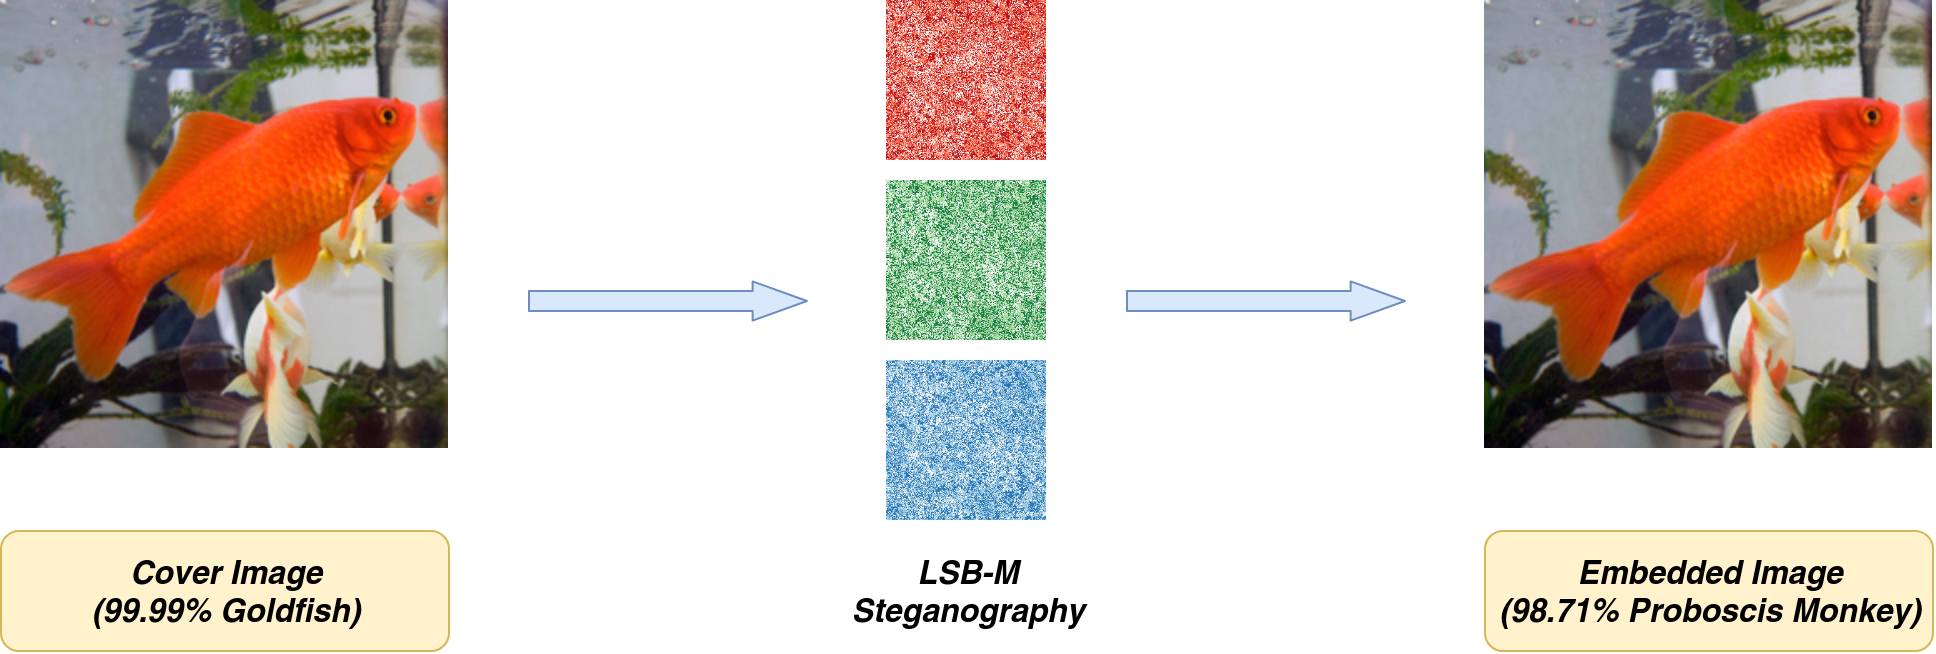
\includegraphics[width=0.9\columnwidth]{images/Steganography-Distortion/Steganography-Distortion.png}%
  \caption{LSB-Matching Embedded Image Misclassification}%
  \label{fig:steganography_distortion}
  \vspace{\baselineskip}
  The cover image and embedded image both use ImageNet pretrained ResNet-18~\cite{ResNet} network for classification. The percentage before the predicted class label represents network's confidence in prediction. The red, green and blue noisy images in the center represent the altered pixel locations in corresponding channels during steganography. There're only three kinds of colors within these images where white stands for no modification, the lighter one stands for a +1 modification and the darker one stands for a -1 modification.
\end{figure}

\subsection{Related Works}

Most previous steganography models focus on resisting steganalysis algorithms or raising embedding payload capacity. BPCS~\cite{BPCS2002,BPCS2015} and PVD~\cite{PVD,PVD_LSB,PVD_Mod} uses adaptive embedding based on local complexty to improve embedding visual quality. HuGO~\cite{HUGO} and S-UNIWARD~\cite{S_UNIWARD} resist steganalysis by minimizing a suitably defined distortion function. Hu~\cite{GANStego} adopts deep convolutional generative adversarial network to achieve steganography without embedding. Wu~\cite{StegNet} and Baluja~\cite{HIPS} achieve a vast payload capacity by focusing on image-into-image steganography.

\subsection{Contributions of this work}

In this paper, we propose a Binary Attention Steganography Network (abbreviated as \textbf{BASN}) architecture to achieve a relatively high payload capacity (2--3 bpp, bits per pixel) with minimal distortion to other neural-network-automated tasks. It utilizes convolutional neural networks with two attention mechanisms, which minimizes embedding distortion to the human visual system and neural network feature maps respectively. Additionally, multiple attention fusion strategies are suggested to balance payload capacity with security, and a fine-tuning mechanism are put forward to improve the hidden information extraction accuracy.
